\begin{frame}{One Image, Many Scenes}
  \begin{columns}[T,onlytextwidth]
    \column{0.46\textwidth}
      \centering
      \vspace{0.8em}
      % Ray slope 1/4: object tops (2,0.5), (4,1), (6,1.5) and the image point (1,0.25) all lie on y = x/4.
      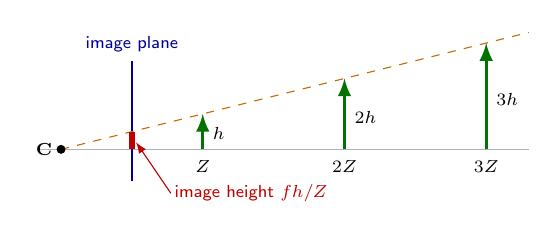
\begin{tikzpicture}[font=\sffamily\scriptsize, >=latex, scale=0.9, every node/.style={transform shape}]
        \draw[gray!60] (-0.3,0) -- (6.6,0);
        \draw[thick, blue!60!black] (1,-0.45) -- (1,1.25) node[above] {image plane};
        \draw[dashed, orange!80!black] (0,0) -- (6.6,1.65);
        \fill (0,0) circle (1.8pt) node[left] {$\mathbf{C}$};
        \draw[->, very thick, green!45!black] (2,0) -- (2,0.5);
        \draw[->, very thick, green!45!black] (4,0) -- (4,1.0);
        \draw[->, very thick, green!45!black] (6,0) -- (6,1.5);
        \node[right] at (2.02,0.22) {$h$};
        \node[right] at (4.02,0.45) {$2h$};
        \node[right] at (6.02,0.7) {$3h$};
        \node[below] at (2,-0.03) {$Z$};
        \node[below] at (4,-0.03) {$2Z$};
        \node[below] at (6,-0.03) {$3Z$};
        \draw[line width=2.2pt, red!75!black] (1,0) -- (1,0.25);
        \draw[->, red!75!black] (1.55,-0.62) node[right, xshift=-2pt] {image height $fh/Z$} -- (1.06,0.1);
      \end{tikzpicture}\\[0.8em]
      {\scriptsize Camera centre $\mathbf{C}$, image plane at focal length $f$. Objects of height $h$, $2h$, $3h$ at depths $Z$, $2Z$, $3Z$ give the same image, because the image height is $fh/Z$.\par}
    \column{0.52\textwidth}
      \begin{itemize}\footnotesize\itemsep0.3em
        \item \textbf{Ill-posed:} back-projection gives only a ray, $\mathbf{X}_c = Z\,K^{-1}\tilde{\mathbf{x}}$, and scaling the whole scene by any $\alpha>0$ leaves every pixel unchanged, so one image cannot fix $Z$.
        \item \textbf{Monocular cues:} perspective (parallel lines converge), relative and familiar size, texture gradient (a uniform texture looks denser farther away), occlusion, shading, defocus blur, and height in the image (on a ground plane, farther points lie closer to the horizon).
        \item \textbf{Learned reliably:} depth ordering (what occludes what) and scene shape up to a global scale.
        \item \textbf{Absolute scale:} only through priors on familiar object sizes and on the camera; a network trained on one camera inherits its scale.
        \item Most of the scenes that fit an image are physically implausible, yet ``At least one major ambiguity remains, though: the global scale.''
      \end{itemize}
      \vspace{0.1em}
      {\scriptsize Quotation: Eigen et al., NIPS 2014, \href{https://arxiv.org/abs/1406.2283v1}{arXiv:1406.2283v1}, Section~1.\par}
  \end{columns}
\end{frame}

\begin{frame}{Supervised Depth and the Scale-Invariant Loss}
  \begin{columns}[T,onlytextwidth]
    \column{0.54\textwidth}
      \begin{itemize}\footnotesize\itemsep0.3em
        \item \textbf{Two networks:} a coarse network (five convolution and pooling layers, then two fully connected layers) predicts the depth layout from the whole image; a fine network refines it locally, taking the coarse map as an extra feature map. The output is log depth.
        \item \textbf{Scale-invariant loss} with $e_i = \ln y_i - \ln y_i^*$:
        \[ L = \frac{1}{n}\sum_i e_i^2 \;-\; \frac{\lambda}{n^2}\Big(\sum_i e_i\Big)^2, \qquad \lambda\in[0,1] \]
        $y_i$ is the predicted and $y_i^*$ the ground-truth depth at pixel $i$; $n$ counts the pixels that have ground truth.
        \item $\lambda=0$ is the per-pixel $\ell_2$ error in log space. $\lambda=1$ is exactly scale-invariant: it equals that error after the best global rescaling of $y$. Training used $\lambda=0.5$, which kept good absolute scale.
      \end{itemize}
    \column{0.44\textwidth}
      \begin{tcolorbox}[colframe=KAred, colback=gray!6, boxrule=0.5pt, left=4pt, right=4pt, top=3pt, bottom=3pt]
        \footnotesize\textbf{Worked example.} Predict $y_i = 2\,y_i^*$ at every pixel. Then $e_i = \ln 2 \approx 0.69$ for all $i$, and
        \[ L = (1-\lambda)(\ln 2)^2 = \begin{cases} 0.48 & \lambda=0\\ 0.24 & \lambda=0.5\\ 0 & \lambda=1 \end{cases} \]
      \end{tcolorbox}
      \begin{itemize}\footnotesize\itemsep0.3em
        \item \textbf{Labels:} NYU Depth v2 records 464 indoor scenes as Microsoft Kinect video; KITTI projects a car-mounted rotating LiDAR into the camera.
        \item \textbf{Sparse and noisy:} reprojected LiDAR covers under 5\% of KITTI pixels, and Kinect depth has holes at windows, specular surfaces, and object boundaries. Pixels without depth are masked out of the loss.
      \end{itemize}
  \end{columns}
  \vspace{0.2em}
  {\scriptsize Eigen et al., NIPS 2014, \href{https://arxiv.org/abs/1406.2283v1}{arXiv:1406.2283v1}, Sections~3--4, Eqs.~3--4; LiDAR coverage: Godard et al., CVPR 2017, \href{https://arxiv.org/abs/1609.03677v3}{arXiv:1609.03677v3}, Section~4.\par}
\end{frame}

\begin{frame}{Self-Supervision from Video: View Synthesis}
  \centering
  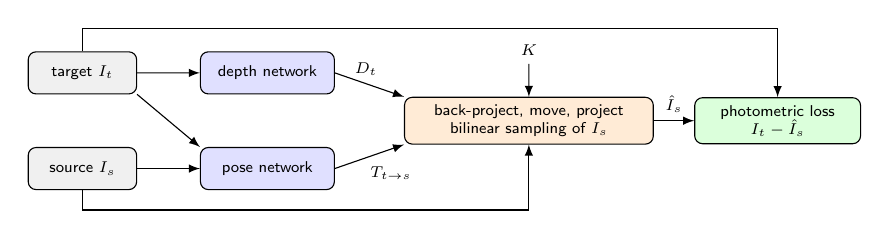
\begin{tikzpicture}[font=\sffamily\scriptsize, >=latex, scale=0.81, every node/.style={transform shape},
      box/.style={draw, rounded corners=0.1cm, align=center, minimum height=0.66cm},
      img/.style={box, fill=gray!12, minimum width=1.7cm},
      net/.style={box, fill=blue!12, minimum width=2.1cm},
      geo/.style={box, fill=orange!16, minimum width=3.9cm},
      lossbox/.style={box, fill=green!14, minimum width=2.6cm}]
    \node[img] (it) at (0,1.15) {target $I_t$};
    \node[img] (is) at (0,-0.35) {source $I_s$};
    \node[net] (dn) at (2.9,1.15) {depth network};
    \node[net] (pn) at (2.9,-0.35) {pose network};
    \node[geo] (warp) at (7.0,0.4) {back-project, move, project\\bilinear sampling of $I_s$};
    \node[lossbox] (loss) at (10.9,0.4) {photometric loss\\$\lvert I_t - \hat{I}_s\rvert$};
    \node (kk) at (7.0,1.5) {$K$};
    \draw[->] (it) -- (dn);
    \draw[->] (it.south east) -- (pn.north west);
    \draw[->] (is) -- (pn);
    \draw[->] (dn.east) -- node[above, pos=0.45] {$D_t$} (warp.north west);
    \draw[->] (pn.east) -- node[below right, pos=0.4] {$T_{t\to s}$} (warp.south west);
    \draw[->] (kk) -- (warp.north);
    \draw[->] (is.south) -- (0,-1.0) -| (warp.south);
    \draw[->] (warp) -- node[above] {$\hat{I}_s$} (loss);
    \draw[->] (it.north) -- (0,1.85) -| (loss.north);
  \end{tikzpicture}\\[0.15em]
  {\scriptsize Training graph of Zhou et al.\ in this lecture's notation ($I_s$: $I_{t\pm1}$). To predict depth at test time, only the depth network runs.\par}
  \begin{columns}[T,onlytextwidth]
    \column{0.49\textwidth}
      \begin{itemize}\footnotesize\itemsep0.2em
        \item \textbf{Warp:} back-project pixel $\mathbf{p}_t$ with its predicted depth, move it by $T_{t\to s}$ (rotation $R$, translation $\mathbf{t}$), and project it into the source:
        \[ \tilde{\mathbf{p}}_s \sim K\big(R\,D_t(\mathbf{p}_t)\,K^{-1}\tilde{\mathbf{p}}_t + \mathbf{t}\big) \]
        \item \textbf{Bilinear sampling} reads $I_s$ at the non-integer point $\mathbf{p}_s$ to give $\hat{I}_s(\mathbf{p}_t)$, and is differentiable in $D_t$ and $T_{t\to s}$.
      \end{itemize}
    \column{0.49\textwidth}
      \begin{itemize}\footnotesize\itemsep0.2em
        \item \textbf{No depth labels:} the photometric loss trains both networks. It assumes a static scene, no occlusion, and Lambertian surfaces (brightness independent of viewpoint).
        \item \textbf{Scale:} the scale ambiguity remains: $D_t$ and $\mathbf{t}$ can grow together without moving $\tilde{\mathbf{p}}_s$, so video gives depth only up to scale.
        \item \textbf{Stereo pairs} (Godard et al., 2017): the source is the other rectified camera, and the known baseline $B$ gives metric depth via $Z = fB/d$.
      \end{itemize}
  \end{columns}
  \vspace{0.1em}
  {\raggedright\scriptsize Zhou et al., ``Unsupervised Learning of Depth and Ego-Motion from Video,'' CVPR 2017, \href{https://arxiv.org/abs/1704.07813v2}{arXiv:1704.07813v2}, Sections~3.1--3.3; Godard et al., \href{https://arxiv.org/abs/1609.03677v3}{arXiv:1609.03677v3}, Section~3.\par}
\end{frame}

\begin{frame}{Monodepth2: Making the Photometric Loss Work}
  \begin{columns}[T,onlytextwidth]
    \column{0.55\textwidth}
      \begin{itemize}\footnotesize\itemsep0.2em
        \item \textbf{Photometric error} between the target and a warped source, with $\alpha = 0.85$:
        \[ pe(I_a, I_b) = \frac{\alpha}{2}\big(1-\text{SSIM}(I_a,I_b)\big) + (1-\alpha)\lVert I_a - I_b\rVert_1 \]
        \item \textbf{SSIM} (structural similarity) compares patches $x$ and $y$ in a small window:
        \[ \text{SSIM}(x,y)=\frac{(2\mu_x\mu_y+C_1)(2\sigma_{xy}+C_2)}{(\mu_x^2+\mu_y^2+C_1)(\sigma_x^2+\sigma_y^2+C_2)} \]
        $\mu$, $\sigma^2$: local means and variances; $\sigma_{xy}$: covariance; $C_1, C_2$: small constants. SSIM is 1 only for identical patches.
      \end{itemize}
    \column{0.43\textwidth}
      \centering
      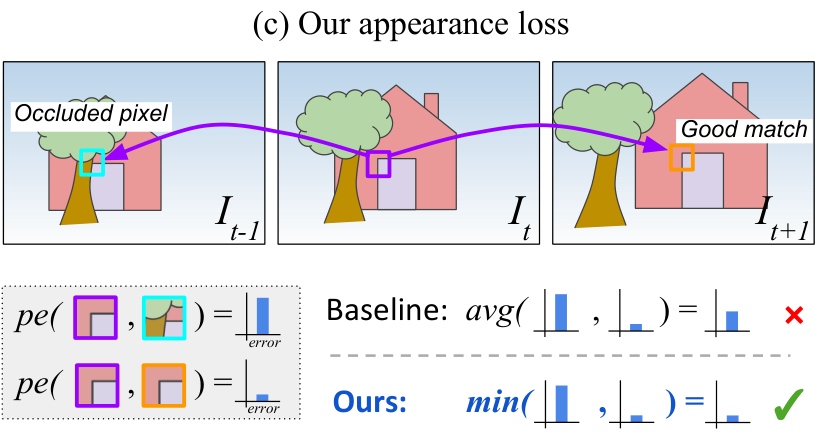
\includegraphics[width=\linewidth,height=0.36\textheight,keepaspectratio]{images/3d-vision/monodepth2_fig3c_min_reprojection.png}\\[0.2em]
      {\scriptsize Godard et al., ``Digging Into Self-Supervised Monocular Depth Estimation,'' ICCV 2019, \href{https://arxiv.org/abs/1806.01260v4}{arXiv:1806.01260v4}, Figure~3(c); losses from Section~3.\par}
  \end{columns}
  \begin{itemize}\footnotesize\itemsep0.2em
    \item \textbf{Per-pixel minimum:} $L_p = \min_s pe(I_t, \hat{I}_s)$, so a pixel occluded in one source is matched in the other.
    \item \textbf{Auto-masking:} keep a pixel only if $\min_s pe(I_t,\hat{I}_s) < \min_s pe(I_t, I_s)$, which drops static-camera frames and objects moving with the camera (otherwise holes of infinite depth).
    \item \textbf{Full-resolution multi-scale:} every decoder scale's depth is upsampled to the input resolution before warping, which reduces holes and texture-copy artifacts (image detail wrongly copied into the depth map).
  \end{itemize}
  {\scriptsize SSIM: Wang et al., IEEE TIP 2004, \href{https://doi.org/10.1109/TIP.2003.819861}{doi:10.1109/TIP.2003.819861}, Eq.~13.\par}
\end{frame}

\begin{frame}{Relative Depth: Scale-and-Shift Invariance}
  \begin{columns}[T,onlytextwidth]
    \column{0.53\textwidth}
      \begin{itemize}\footnotesize\itemsep0.2em
        \item \textbf{Mixed labels:} metric (laser, calibrated stereo), up to scale (multi-view reconstruction), or disparity up to scale and shift (uncalibrated stereo, 3D films).
        \item \textbf{MiDaS} predicts disparity $d_i$ (inverse depth) and fits a scale $s$ and shift $t$ to the ground truth $d_i^*$ by least squares before scoring its $M$ valid pixels:
        \[ \mathcal{L}_{\text{ssi}}=\min_{s,t}\ \frac{1}{2M}\sum\nolimits_{i=1}^{M}\big(s\,d_i+t-d_i^*\big)^2 \]
        Training instead centres both maps on their medians, scales each by its mean absolute deviation, and drops the largest 20\% of residuals from an $\lvert x\rvert$ loss.
      \end{itemize}
    \column{0.45\textwidth}
      \centering
      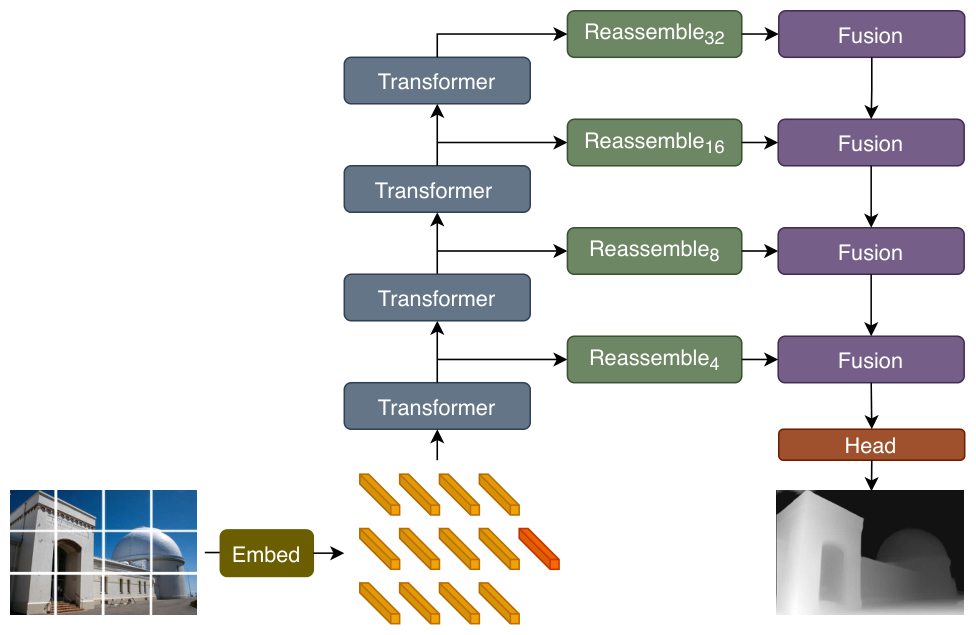
\includegraphics[width=\linewidth,height=0.44\textheight,keepaspectratio]{images/3d-vision/dpt_fig1_architecture.png}\\[0.2em]
      {\scriptsize Ranftl et al., ``Vision Transformers for Dense Prediction,'' ICCV 2021, \href{https://arxiv.org/abs/2103.13413v1}{arXiv:2103.13413v1}, Figure~1 (left); training data: Section~4.1.\par}
  \end{columns}
  \begin{itemize}\footnotesize\itemsep0.1em
    \item \textbf{MiDaS mixes five datasets} Pareto-optimally (no dataset's loss can fall without another's rising); zero-shot tests on six unseen datasets.
    \item \textbf{DPT} (dense prediction transformer, right): tokens from four ViT stages are reassembled into maps at $1/32$ to $1/4$ resolution and fused by a convolutional decoder; MiDaS loss, about 1.4M images.
    \item \textbf{Depth Anything} scaled this recipe with pseudo-labels on 62M unlabeled images.
  \end{itemize}
  {\scriptsize Ranftl et al., TPAMI 2022, \href{https://arxiv.org/abs/1907.01341v3}{arXiv:1907.01341v3}, Sections~3--6; Yang et al., \href{https://arxiv.org/abs/2401.10891v2}{arXiv:2401.10891v2}, Section~3.\par}
\end{frame}

\begin{frame}{Metric Depth from a Single Image}
  \begin{itemize}\footnotesize\itemsep0.2em
    \item \textbf{The camera sets the scale:} an object's image height $fh/Z$ is the same with focal length $2f$ at depth $2Z$, so without $f$ the image size cannot separate the two depths.
    \item \textbf{Metric3D} maps each training image to a canonical camera with focal length $f^c$, scaling the depth label (or resizing the image) by $f^c/f$ and inverting this at test time; 8M images from 11 datasets (v2: surface normals, 16M images).
    \item \textbf{UniDepth} predicts a dense map of camera ray angles (azimuth, elevation) that conditions the depth module, and outputs a 3D point per pixel.
    \item \textbf{Depth Pro} predicts a canonical inverse depth $C$ and returns $D_m = f_{px}/(wC)$ ($f_{px}$: focal length in pixels, $w$: image width); a separate head predicts the field of view. A 2.25-megapixel map takes 0.3\,s on a V100.
  \end{itemize}
  \vspace{0.1em}
  {\centering\scriptsize
  \begin{tabular}{>{\raggedright\arraybackslash}p{2.8cm} >{\raggedright\arraybackslash}p{6.0cm} >{\raggedright\arraybackslash}p{3.2cm}}
    \toprule
    \textbf{Method} & \textbf{Source of metric scale} & \textbf{Camera at test time} \\
    \midrule
    Supervised, one dataset & metric labels from one sensor and camera & same camera as training \\
    \addlinespace[0.1em]
    Stereo self-supervision & baseline $B$ and focal length $f$ of the training rig & same camera as training \\
    \addlinespace[0.1em]
    Metric3D, Metric3D v2 & canonical camera: labels or images rescaled by $f^c/f$ & focal length required \\
    \addlinespace[0.1em]
    UniDepth & predicted per-pixel camera rays & none (optional input) \\
    \addlinespace[0.1em]
    Depth Pro & canonical inverse depth and a predicted focal length & none \\
    \bottomrule
  \end{tabular}\par}
  \vspace{0.2em}
  {\scriptsize Yin et al., ICCV 2023, \href{https://arxiv.org/abs/2307.10984v1}{arXiv:2307.10984v1}, Sections~1, 3.1--3.2, 4; Hu et al., TPAMI 2024, \href{https://arxiv.org/abs/2404.15506v4}{arXiv:2404.15506v4}; Piccinelli et al., CVPR 2024, \href{https://arxiv.org/abs/2403.18913v1}{arXiv:2403.18913v1}; Bochkovskii et al., ICLR 2025, \href{https://arxiv.org/abs/2410.02073v2}{arXiv:2410.02073v2}, Sections~1, 3.2--3.3.\par}
\end{frame}

\begin{frame}{Diffusion Priors for Depth}
  \begin{columns}[T,onlytextwidth]
    \column{0.54\textwidth}
      \begin{itemize}\footnotesize\itemsep0.25em
        \item \textbf{Marigold} turns Stable Diffusion v2 into a depth estimator. The frozen VAE encodes the image $\mathbf{x}$ and the depth map $\mathbf{d}$ (copied to three channels).
        \item The U-Net input is the image latent concatenated with the noisy depth latent; only the U-Net is fine-tuned (usual denoising objective, no text prompt).
        \item \textbf{Synthetic data only:} about 54K Hypersim (indoor) and 20K Virtual KITTI (street) samples with dense, noise-free depth, each normalised by its 2nd and 98th percentiles: the output is affine-invariant (fixed only up to an unknown scale and shift).
        \item \textbf{Inference:} 50 DDIM steps from noise, then the VAE decoder. Ten runs from different noise are aligned in scale and shift and merged by the pixelwise median, which cuts the absolute relative error (the mean of $\lvert y_i-y_i^*\rvert/y_i^*$) on NYU Depth v2 by 8\%.
        \item \textbf{Cost:} about 2.5 days of fine-tuning on one RTX 4090 GPU.
      \end{itemize}
    \column{0.44\textwidth}
      \centering
      \vspace{1.0em}
      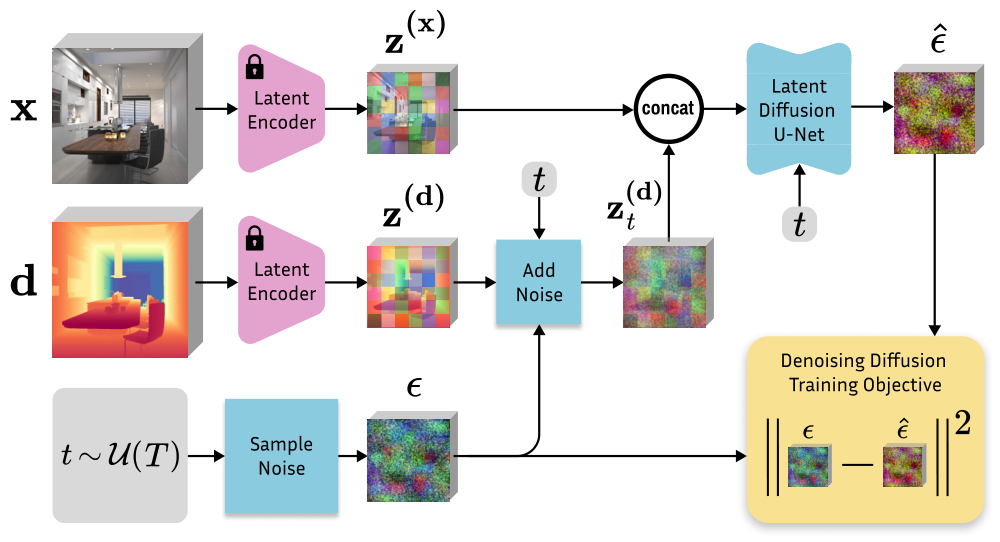
\includegraphics[width=\linewidth,height=0.52\textheight,keepaspectratio]{images/3d-vision/marigold_fig2_finetuning.png}\\[0.2em]
      {\scriptsize ``Overview of the Marigold fine-tuning protocol.'' Ke et al., ``Repurposing Diffusion-Based Image Generators for Monocular Depth Estimation,'' CVPR 2024, \href{https://arxiv.org/abs/2312.02145v2}{arXiv:2312.02145v2}, Figure~2; numbers from Sections~3--4.\par}
  \end{columns}
\end{frame}

\begin{frame}{Evaluating Depth: Metrics and Protocols}
  \begin{itemize}\footnotesize\itemsep0.2em
    \item AbsRel is the absolute relative error; over the $N$ pixels with ground-truth depth $y_i^*$ and predicted depth $y_i$,
    \[ \textstyle \text{RMSE}=\sqrt{\frac{1}{N}\sum_i (y_i-y_i^*)^2} \]
    $\delta_1$: fraction of pixels with $\max(y_i/y_i^*,\, y_i^*/y_i) < 1.25$ ($\delta_2$, $\delta_3$: $1.25^2$, $1.25^3$); higher is better.
    \item \textbf{NYU Depth v2:} 654 indoor test images from a Kinect, evaluated up to 10\,m.
    \item \textbf{KITTI Eigen split:} 697 test images from 29 scenes, reprojected LiDAR, a fixed crop, depth capped at 80\,m. Marigold uses a 652-image version; 652 of the 697 frames have improved ground truth.
  \end{itemize}
  {\footnotesize Alignment uses the ground truth, so compare scores only within one protocol:\par}
  \vspace{0.15em}
  {\centering\scriptsize\setlength{\tabcolsep}{4pt}
  \begin{tabular}{>{\raggedright\arraybackslash}p{2.6cm} >{\raggedright\arraybackslash}p{5.6cm} >{\raggedright\arraybackslash}p{4.8cm}}
    \toprule
    \textbf{Protocol} & \textbf{Used for} & \textbf{Alignment before scoring} \\
    \midrule
    Median scaling & self-supervised monocular models & $y \leftarrow y\cdot\text{median}(y^*)/\text{median}(y)$ per image \\
    \addlinespace[0.1em]
    Least-squares scale and shift & affine-invariant models (MiDaS, DPT, Marigold) & fit $s, t$ on valid pixels (in disparity for disparity models) \\
    \addlinespace[0.1em]
    No alignment & metric models (Metric3D, UniDepth, Depth Pro) & none: the prediction is scored as it is \\
    \bottomrule
  \end{tabular}\par}
  \vspace{0.15em}
  {\scriptsize Metrics: Eigen et al., \href{https://arxiv.org/abs/1406.2283v1}{arXiv:1406.2283v1}, Section~4.3. Protocols: Zhou et al., \href{https://arxiv.org/abs/1704.07813v2}{arXiv:1704.07813v2}, Section~4.1; Godard et al., \href{https://arxiv.org/abs/1806.01260v4}{arXiv:1806.01260v4}, Section~4.1 and supplementary D.1 (improved ground truth); Ranftl et al., \href{https://arxiv.org/abs/1907.01341v3}{arXiv:1907.01341v3}, Section~6. Splits: Godard et al., \href{https://arxiv.org/abs/1609.03677v3}{arXiv:1609.03677v3}, Section~4; Ke et al., \href{https://arxiv.org/abs/2312.02145v2}{arXiv:2312.02145v2}, Section~4.2.\par}
\end{frame}
